\documentclass{beamer}

\usepackage[utf8]{inputenc}
\usepackage[T1]{fontenc}
\usepackage[slovene]{babel}
\usepackage{lmodern}
\usepackage{array}     
\usepackage{tikz}

\usetheme{CambridgeUS}
\usecolortheme{rose}
\useinnertheme{rounded}
\useoutertheme{infolines}
\beamertemplatenavigationsymbolsempty

\usepackage{palatino}
\usefonttheme{serif}

\begin{document}

%==============================================================================================================================
\title[Principi računanja zavarovalnih premij]{PRINCIPI RAČUNANJA ZAVAROVALNIH PREMIJ}
\subtitle{Zakaj mora čista premija presegati pričakovano škodo}
\author{Neža Kržan}
\institute[FMF]{Fakulteta za matematiko in fiziko}
\date{}

\begin{frame}
	\titlepage
\end{frame}

%------------------------------------------------------------------------------------------------------------------------------
\section{Zavarovalna premija}
\begin{frame}
	\frametitle{ZAVAROVALNA PREMIJA}
	   \begin{alertblock}{}
		Zavarovalna premija je plačilo za zavarovanje oziroma cena zavarovanja.
	\end{alertblock}
\vspace{0.5cm}
\begin{itemize}
\item<1->Zavarovanec plača bruto premijo.\\
\item<2->Bruto premija se deli na \textbf{čisto premijo} in \textbf{režijski dodatek}.
\end{itemize}
\end{frame}

%------------------------------------------------------------------------------------------------------------------------------
\section{Čista premija}
\begin{frame}
	\frametitle{ČISTA PREMIJA}
	\begin{alertblock}{Trditev:}
		Denimo, da je škoda vsako leto porazdeljena normalno, torej $N(\mu, \sigma ^2)$. Višine škodnih zahtevkov vsako leto so med seboj neodvisne in 
		\begin{itemize}
			\item $K_n$ naj bo kapital n-tega leta,
			\item $z$ naj bo začetni kapital ob letu $0$,
			\item $\mu_i$ je pričakovana vrednost šode i-tega leta ter
			\item $X_i$ naj bo višina škodnega zahtevka v i-tem letu.
		\end{itemize}
		Potem za kapital zavarovalnice v n-tem letu velja:
		\[
		K_n = z + \sum_{i=1}^n (\mu_i - X_i).
		\]
	\end{alertblock}
\end{frame}

%------------------------------------------------------------------------------------------------------------------------------
\section{Verjetnost propada}
\begin{frame}
	\frametitle{VERJETNOST PROPADA}
	\begin{alertblock}{}
		V zavarovalništvu se uporablja teorija propada ali teorija tveganja, ki uporablja matematične modele za opis ranljivosti zavarovalnice za plačilno nesposobnost oziroma propad.
	\end{alertblock}

	\begin{itemize}
	\item<1->Vedno upoštevamo časovni razvoj kapitala $U(t)$ zavarovalnice.
	\item<2->$\psi(u)$ označuje verjetnost, da se propad zavarovalnice zgodi.
	\end{itemize}
\end{frame}

%------------------------------------------------------------------------------------------------------------------------------
\begin{frame}
	\begin{itemize}
		\item<1->Verjetnost propada omogoča primerjavo portfeljev.
		\item<1->Ne moremo pa ji pripisati absolutni pomen verjetnosti uničenja.
	\end{itemize}
\vspace{0.5cm}
	\begin{alertblock}{}
		Dejansko ne predstavlja verjetnosti, da bo zavarovalnica propadla.
	\end{alertblock}
	\begin{itemize}
		\item Traja lahko več stoletij, da se propad zgodi.
		\item Očitni posegi v proces so izključeni pri opredelitvi verjetnosti uničenja.
	\end{itemize}
\end{frame}

%------------------------------------------------------------------------------------------------------------------------------
\begin{frame}
	\frametitle{APROKSIMACIJA VERJETNOSTI PROPADA}
	\begin{alertblock}{}
		Za verjetnostne porazdelitve je težko najti točno vrednost verjetnosti propada $\psi(u)$, zato potrebujemo dobre in preproste približke za verjetnost propada.
	\end{alertblock}

Predstavila vam bom šest možnih aproksimacij.
\end{frame}

%------------------------------------------------------------------------------------------------------------------------------
\begin{frame}
	\frametitle{Aproksimacija verjetnosti propada}
	Za aproksimacijsko funkcijo vzamemo
	\[
	\psi(u) \approx \frac{1}{1 + \theta} e^{-Ru}.
	\]
	kjer je $R$ koeficient prilagoditve porazdelitve velikosti terjatev.
\end{frame}

%------------------------------------------------------------------------------------------------------------------------------
\begin{frame}
	\frametitle{Aproksimacija verjetnosti propada}
	Pri prejšni aproksimaciji lahko vzamemo tudi natančno verjetnost propada porazdeljeno eksponentno s koeficientom prilagoditve R, kar je
	\[
	\psi(u) \approx (1 - R\mu_1)e^{-Ru}.
	\]
\end{frame}

%------------------------------------------------------------------------------------------------------------------------------
\begin{frame}
	\frametitle{Aproksimacija verjetnosti propada}
	Če zamenjamo porazdelitev terjatev z eksponentno porazdelitvijo z enako pričakovano vrednostjo, dobimo
	\[
	\psi(u) \approx \frac{1}{1 + \theta} exp(-\frac{\theta}{1+ \theta}\frac{u}{\mu_1}).
	\]
\end{frame}

%------------------------------------------------------------------------------------------------------------------------------
\begin{frame}
	\frametitle{Aproksimacija verjetnosti propada}
	Če $\psi(u)$ aproksimiramo z $\psi(0)e^{-ku}$, kjer je $k$ tak, da velja 
	\[ \int_{0}^{\infty} \psi(u) du = \frac{\mu_2}{2\theta \mu_1}\]
	za aproksimacijo 
	\[
	\psi(u) \approx \frac{1}{1 + \theta} exp(\frac{-2\theta \mu_1 u}{(1 + \theta)\mu_2}).
	\]
\end{frame}

%------------------------------------------------------------------------------------------------------------------------------
\begin{frame}
	\frametitle{Aproksimacija verjetnosti propada}
	Še ena možnost je aproksimacija z diskretno porazdelitvijo.
	\vspace{0.5cm}
	\\Če pa verjetnost propada aproksimiramo z geometrijsko porazdelitvijo, nam ta omogoča uporabo Panjerjeve rekurzije, če so posamezni členi celoštevilski.
\end{frame}

%------------------------------------------------------------------------------------------------------------------------------
\section{Principi računanja zavarovalnih premij}
\begin{frame}
	\frametitle{PRINCIPI RAČUNANJA ZAVAROVALNIH PREMIJ}
	Princip premije je dobro definirano pravilo za izračun premije za dano tveganje, ki pa je slučajna spremenljivka. \\
	\vspace{0.5cm}
	Premija vključuje tako proces tveganja kot parameter tveganja, provizije in stroški pa so izločeni iz principa premije.
\end{frame}

%------------------------------------------------------------------------------------------------------------------------------
\begin{frame}
	\frametitle{IZRAČUN PREMIJE OD ZGORAJ NAVZDOL}
	\begin{columns}[c]
		\begin{column}{0.60\textwidth}
			\begin{itemize}
				\item Hans Bühlmann je opisal pristop od zgodraj navzdol za izračun premij.
				\item Rezultat je eksponentna premija, pri čemer parameter nenaklonjenosti tveganju $\alpha$  izhaja iz največje dovoljene verjetnosti propada in razpoložljivega začetnega kapitala.
			\end{itemize}
		\end{column}
		\begin{column}{0.40\textwidth}
			\centering
			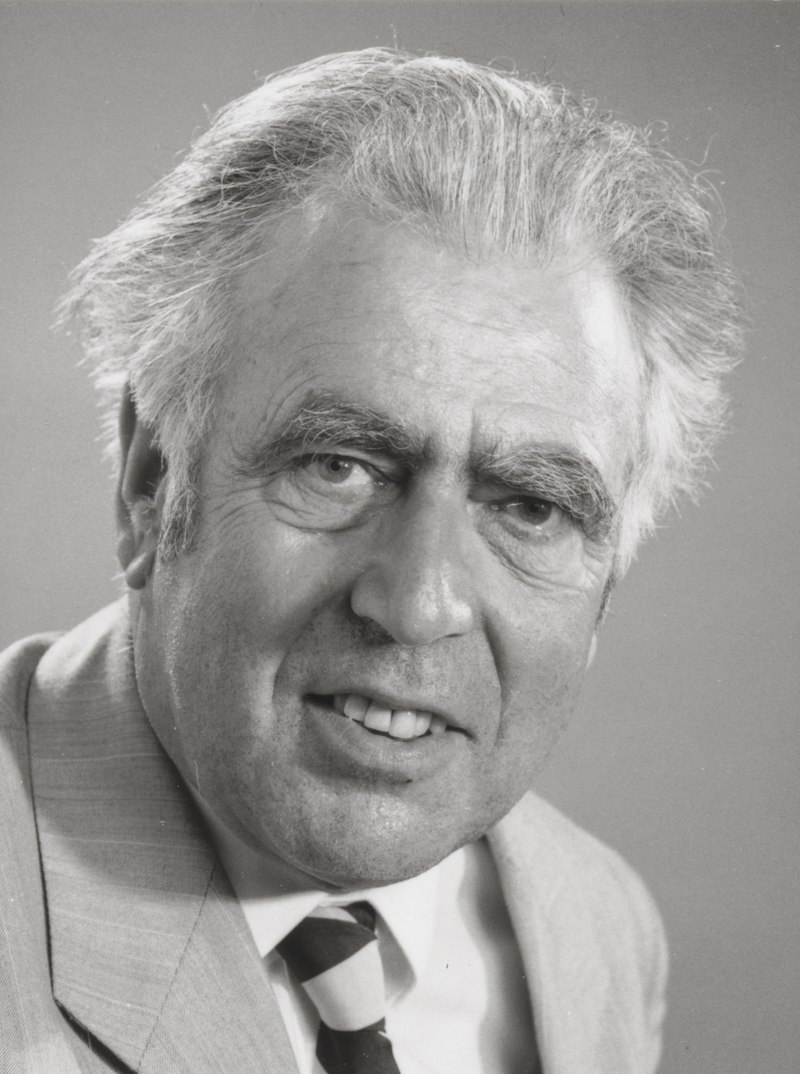
\includegraphics[scale=0.15]{hans.jpg}
			Hans Bühlmann
		\end{column}
	\end{columns}
\end{frame}

%------------------------------------------------------------------------------------------------------------------------------
\section{Simulacija}
\begin{frame}
	\frametitle{SIMULACIJA}
	\begin{itemize}
		\item Imamo več zavarovalnic z isto količino začetnega kapitala.
		\item Vsaka od njih z verjetnostjo $50 \%$ pridobi ali z verjetnostjo $50 \%$ izgubi eno enoto kapitala.
		\item Določimo začetno količino kapitala, število zavarovalnic in število let.
	\end{itemize}
\end{frame}

%------------------------------------------------------------------------------------------------------------------------------
\begin{frame}
	\frametitle{ZAČETNI MODEL}
	\begin{itemize}
		\item Opazujemo 100 zavarovalnic.
		\item Spreminjamo njihov začetni kapital ter leta opazovanja.
		\item Kapital narašča od 3 do 100 enot, leta pa od 10 pa do 50000.
	\end{itemize}

\begin{table}[htb]
	\centering
	\caption{Deleži propadlih zavarovalnic v odvisnosti od začetnega kapitala}
	\begin{tabular}{|c|c|c|c|c|c|c|c|c|c|c|}
		\hline
		\textbf{z} \backslash \textbf{leta} & \textbf{10} & \textbf{50} & \textbf{100} & \textbf{500} & \textbf{1000} & \textbf{5000} & \textbf{10000} & \textbf{500000} \\\hline
		\textbf{3} & 0.31 & 0.64 & 0.72 & 0.90 & 0.96 & 0.98 & 0.99 & 1 \\\hline
		\textbf{10} & 0 & 0.16 & 0.32  & 0.66 & 0.75 & 0.85 & 0.92 & 1 \\\hline
		\textbf{25} & 0  & 0 & 0.03 & 0.29 & 0.45 & 0.66 & 0.81 & 0.91 \\\hline
		\textbf{50} & 0 & 0 & 0 & 0.05 & 0.09 & 0.47 & 0.64 & 0.93 \\\hline
		\textbf{100} & 0 & 0 & 0 & 0 & 0.01 & 0.19 & 0.31 & 0.88 \\\hline
	\end{tabular}
	\label{tab:my_label}
\end{table}
\end{frame}
%------------------------------------------------------------------------------------------------------------------------------
\begin{frame}
	\frametitle{ZAČETNI KAPITAL}
	Verjetnost propada lahko zelo zmanjšamo že z majhnim povečanjem začetnega kapitala.
	\begin{center}
		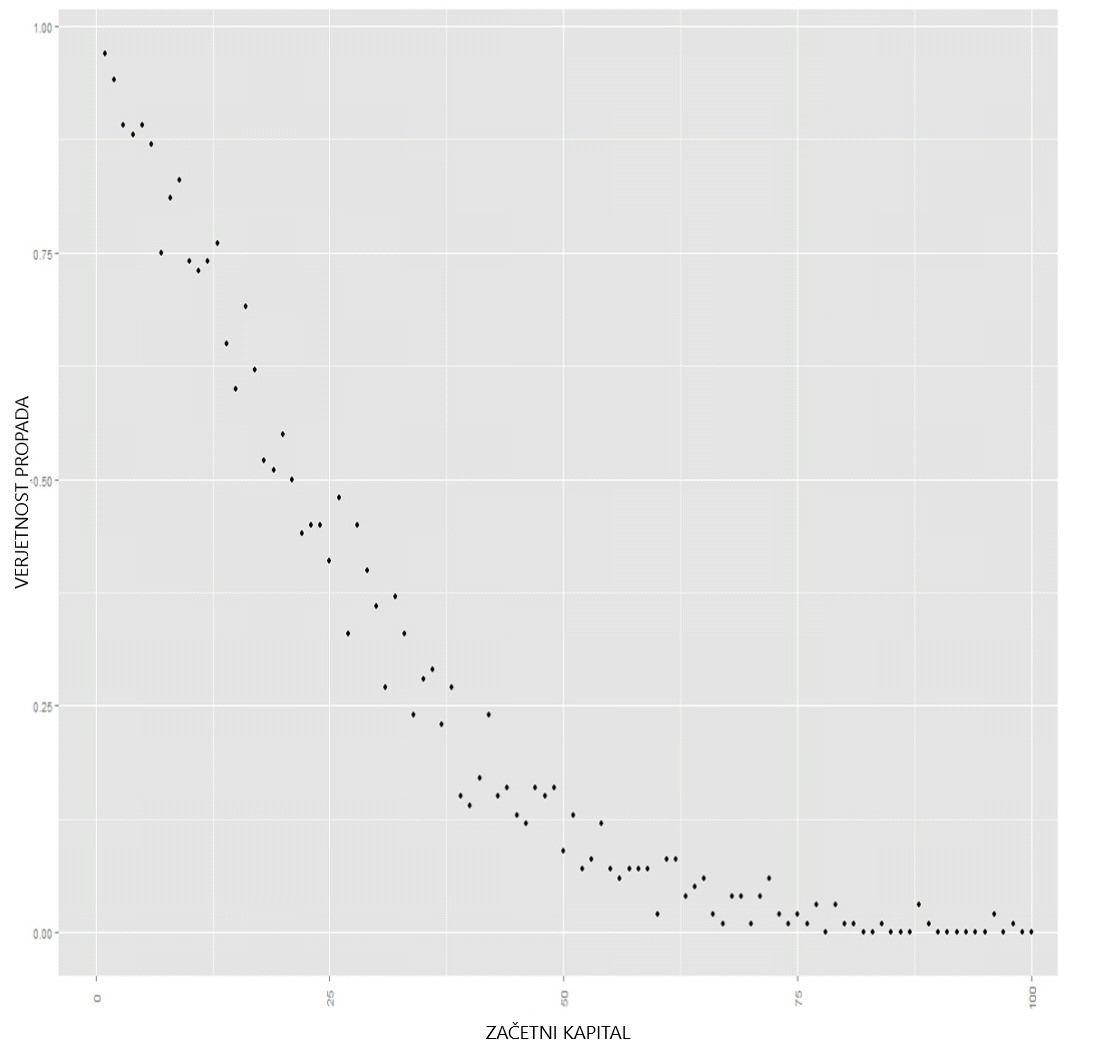
\includegraphics[scale=0.23]{graf1.jpg}  
	\end{center}
\end{frame}

%------------------------------------------------------------------------------------------------------------------------------
\begin{frame}
	\frametitle{NA DOLGI ROK JE VERJETNOST PROPADA 1}
	Kljub poljubnemu povečanju začetnega kapitala se na dolgi rok ne moremo zavarovati pred propadom.
	\begin{center}
		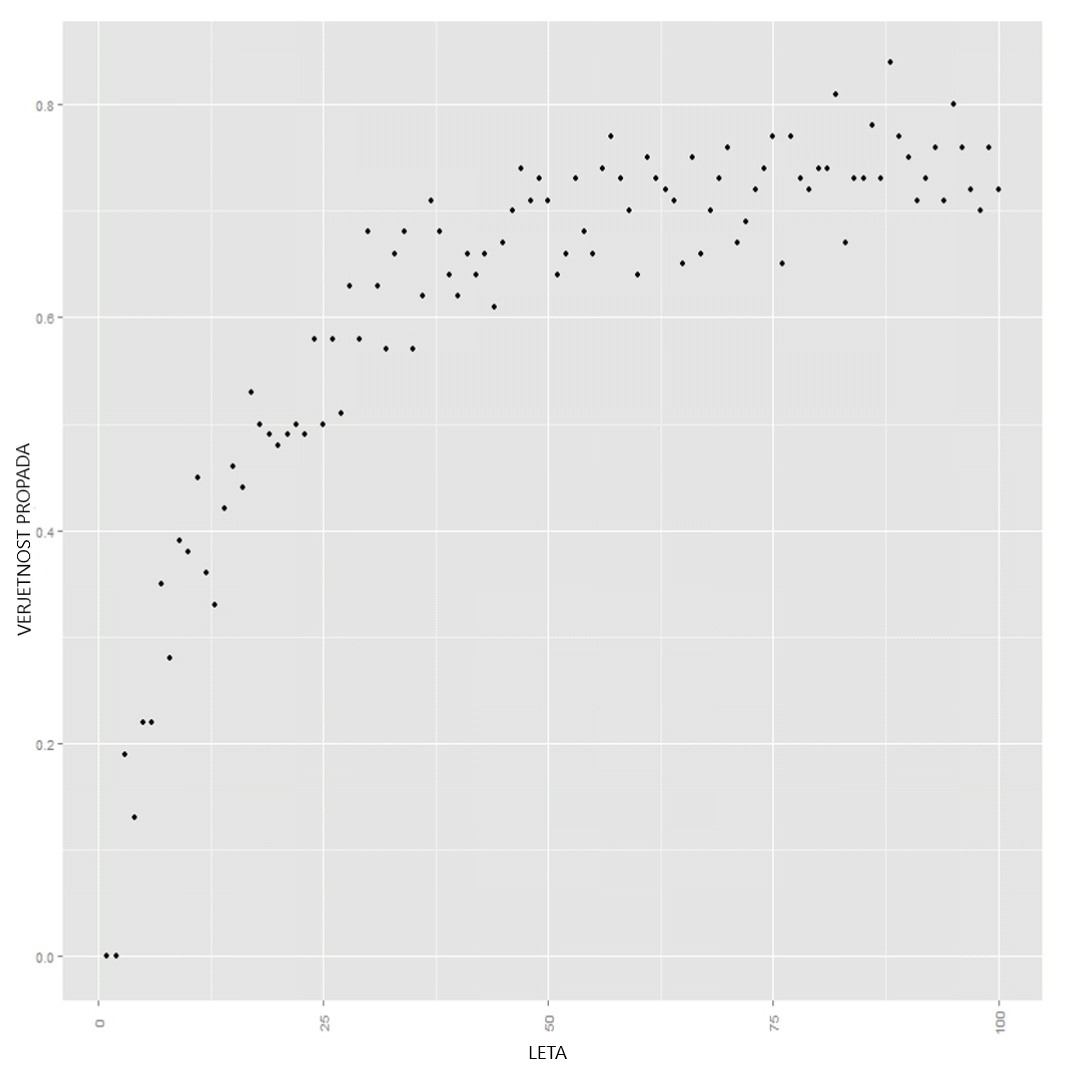
\includegraphics[scale=0.23]{graf3.jpg}  
	\end{center}
\end{frame}

%------------------------------------------------------------------------------------------------------------------------------
\begin{frame}
	\frametitle{SPREMENJENE VERJETNOSTI}
	Zavarovalnici sem povečala čisto premijo. \\
	\vspace{0.2cm}
	Verjetnost slabega stanja je še vedno $50\%$, vendar se takrat kapital zavarovalnice zmanjša za $0.5$, v dobrem stanju pa se poveča za $1.5$ enote. Sedaj se verjetnost propda zavarovalnice zmanjša skoraj na nič.\\
	\vspace{0.2cm}
	Zavarovalnica bo propadla samo v primeru, ko je njen začetni kapital manjši od $5$ enot. 
\end{frame}

%------------------------------------------------------------------------------------------------------------------------------
\begin{frame}
	\frametitle{SPREMENJENE VERJETNOSTI}
	Na naslednjem grafu je kapital fiksiran na $3$ enote, obdobje opazovanja teče od $1$ do $200$ let.
	\begin{center}
		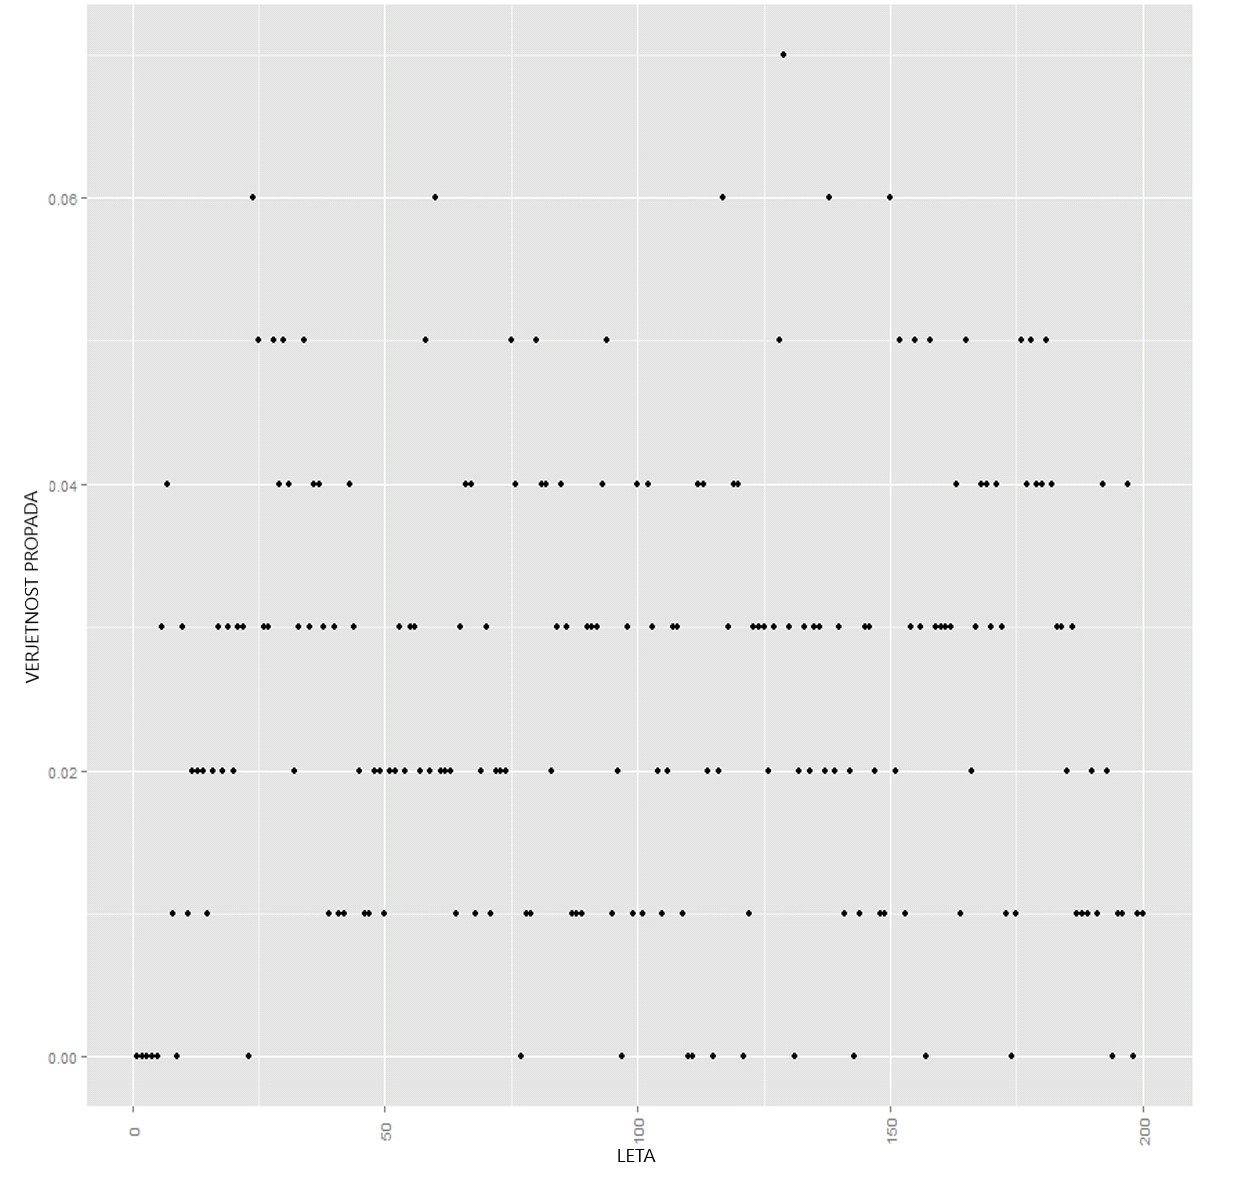
\includegraphics[scale=0.20]{graf2.jpg}  
	\end{center}
\end{frame}

%------------------------------------------------------------------------------------------------------------------------------
\section{Zaključek}
\begin{frame}
	\frametitle{ZAKLJUČEK}
	\begin{alertblock}{}
	Vidimo torej, da mora čista remija presegati matematično upanje pričkovane škode, sicer bo zavarovalnica slej ko prej propadla.
	\end{alertblock}
\end{frame}

\end{document}


